\begin{center}
\makeatletter
\@ifundefined{color@atlasink}{\definecolor{atlasink}{HTML}{33312E}}{}
\@ifundefined{color@atlasgray}{\definecolor{atlasgray}{HTML}{9A958C}}{}
\@ifundefined{color@atlasblue}{\definecolor{atlasblue}{HTML}{2E6F9E}}{}
\@ifundefined{color@atlasgreen}{\definecolor{atlasgreen}{HTML}{4C8C3F}}{}
\@ifundefined{color@atlasred}{\definecolor{atlasred}{HTML}{C0473B}}{}
\@ifundefined{color@atlasgold}{\definecolor{atlasgold}{HTML}{D69A2A}}{}
\@ifundefined{atlascaption}{%
  \newcommand{\atlascaption}[3]{\shortstack{\footnotesize Figure~#1. \textbf{#2:}\\#3}}%
}{}
\@ifundefined{glowstroke}{%
  \newcommand{\glowstroke}[3]{%
    \draw[#1, line width=1.5pt, line cap=round]
      plot[domain=#2,samples=100,smooth] (\x,{#3});%
  }%
}{}
\makeatother
\tikzset{
  atlas axes/.style={atlasink, line width=0.7pt, line cap=round, ->},
  atlas curve/.style={line width=1.5pt, line cap=round, line join=round},
  dropline/.style={atlasgray, line width=0.6pt, dash pattern=on 2pt off 2pt},
  atlas dot/.style={fill=atlasink, draw=white, line width=0.4pt, circle, inner sep=0pt, minimum size=4.2pt},
}

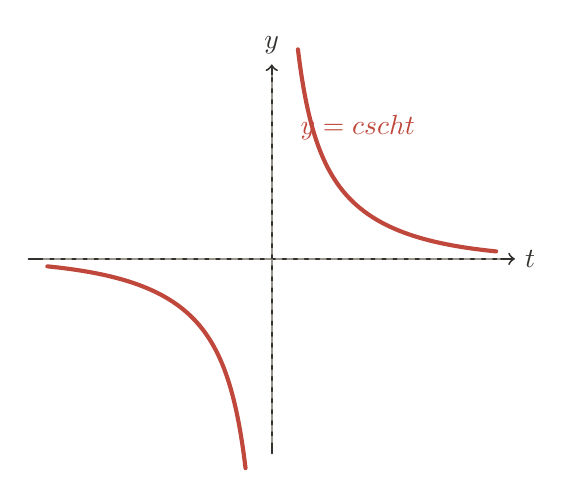
\begin{tikzpicture}[scale=0.95, line cap=round, line join=round]
  \draw[atlas axes] (-3.25,0)--(3.25,0) node[right] {$t$};
  \draw[atlas axes] (0,-2.6)--(0,2.6) node[above] {$y$};
  \draw[dropline] (0,-2.45)--(0,2.45);
  \draw[dropline] (-3.05,0)--(3.05,0);
  \glowstroke{atlasred}{0.35:3}{2/(exp(\x)-exp(-\x))}
  \glowstroke{atlasred}{-3:-0.35}{2/(exp(\x)-exp(-\x))}
  \node[atlasred] at (1.15,1.75) {$y=\operatorname{csch}t$};
\end{tikzpicture}

\atlascaption{H7}{Hyperbolic cosecant}{Odd, undefined at $t=0$, and decays toward $0$.}
\end{center}


\begin{definitionbox}{Definition}
\begin{definition}[Hyperbolic cosecant]
\label{def:hyperbolic-cosecant}
For each $t\in\mathbb{R}\setminus\{0\}$, define the \emph{hyperbolic
cosecant} by
\[
  \operatorname{csch} t=\frac{1}{\sinh t}.
\]
\end{definition}
\end{definitionbox}
\begin{remark*}[Domain and range]
The function $\operatorname{csch}$ is defined on
$\mathbb{R}\setminus\{0\}$ because $\sinh 0=0$. Its range is
$\mathbb{R}\setminus\{0\}$.
\end{remark*}
\begin{dependencies}
\begin{itemize}
  \item \hyperref[def:hyperbolic-sine]{Hyperbolic sine}
\end{itemize}
\end{dependencies}
